\section{Abstract folding}
\frame{\tableofcontents[currentsection]}

\begin{frame}{What kind of folding?}
    \pause
    There are many different kinds of folding (e.\,g. Origami)
    \pause
    Here:
    \begin{itemize}
        \pause
        \item Folding of surface in $\R^3$
        \pause
        \item Possible folding edges are fixed
        \pause
        \item Folding should be rigid (no curvature)
    \end{itemize}

    \pause
    Goal: Classify possible folding patterns (given a net)

    \pause
    \begin{center}
        \movie[ height = 0.4\textwidth, width = 0.4\textwidth, autostart, loop ]{}{TorusNetz.mp4}
    \end{center}

\end{frame}


\begin{frame}{Why are embeddings hard?}
    \pause
    Ideally, we would like to have embeddings.
    
    \pause
    But we want to define folding independently from an embedding, since:

    \begin{itemize}
        \pause
        \item They are very hard to compute (even for small examples)
        \pause
        \item We can only show foldability for specific small examples
            \begin{itemize}
                \pause
                \item Usually using regularity (like crystallographic symmetry)
                \pause
                \item No general method
            \end{itemize}
        \pause
        \item It is very hard to define iterated folding in an embedding
    \end{itemize}

    \pause
    \begin{center}
        \movie[ height = 0.4\textwidth, width = 0.4\textwidth, autostart, loop ]{}{TorusNetz.mp4}
    \end{center}

\end{frame}

%TODO what about forced folding? Or closedness of surfaces under folding? RETHINK this

\begin{frame}{Is there an alternative?}
    \pause
    Central idea:
    \begin{itemize}
        \pause
        \item Don't model folding process (needs embedding)
        \pause
        \item Describe starting and final folding state
            \begin{itemize}
                \pause
                \item Only consider changes in the topology
                    \pause (like identification of faces)
                \pause
                \item allows abstraction from embedding
            \end{itemize}
    \end{itemize}

    % Use pentagon-flippy to illustrate incidence rigidity

    \pause
    $\leadsto$ Incidence geometry (polygonal complex/surface)

    \begin{itemize}
        \pause
        \item Captures some folding restrictions \pause (rigidity of tetrahedron)
        \pause
        \item Still needs a lot of refinement
    \end{itemize}
\end{frame}


\begin{frame}{Important properties of folding}
    \begin{itemize}
        \item<2-> The class of surfaces is not closed under folding
        \item<3-> Folding can be undone by \textit{unfolding}
        \item<4-> Identification of two faces might force identification of two other faces
            \begin{itemize}
                \item<7-> Can apply to arbitrary many faces 
                \item<10-> The forced identification is not unique
                \item<14->[$\Rightarrow$] Identify only two faces at a time
            \end{itemize}
    \end{itemize}

    \begin{overlayarea}{\textwidth}{0.3\textwidth}
        \begin{center}
            \only<5-7|handout:0>{
                % First identification
                \begin{tikzpicture}
                    \def\Hdist{1.5}
	    	    \def\Vdist{1}
			
		    \coordinate (A) at (-\Hdist,0);
		    \coordinate (B) at (0,\Vdist);
		    \coordinate (C) at (\Hdist,0);
		    \coordinate (D) at (0,-\Vdist);
                    \draw (A) -- (B) -- (C) -- (D) -- cycle;

		    \foreach \p in {A,B,C,D}
		        \fill [\vertexColor] (\p) circle (1.5pt);
		    \draw [<->,red,thick] ($(B)!0.5!(A)$) -- ($(D)!0.5!(A)$);
                    \uncover<6-7>{
                        \draw[<->,red,thick] ($(B)!0.5!(C)$) -- ($(D)!0.5!(C)$);
                    }
                \end{tikzpicture}
            }

            % Arbitrary many faces
            \only<8-10|handout:0>{
                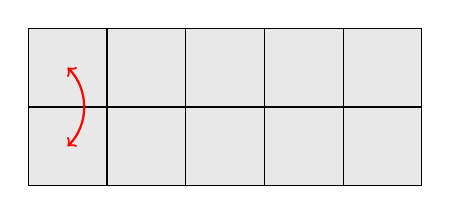
\begin{tikzpicture}
		    \foreach \i/\j in {1/0, 2/1, 3/2, 4/3, 5/4}
		    {
		        \filldraw [fill=black!9!white] (\j,0) -- (\i,0) -- (\i,1) -- (\j,1) -- cycle;
		        \filldraw [fill=black!9!white] (\j,0) -- (\i,0) -- (\i,-1) -- (\j,-1) -- cycle;
		    }
                    \uncover<9-10>{
                        \draw [red,<->,thick] (0.5,0.5) to [out=-45,in=45] (0.5,-0.5);
	            }
                \end{tikzpicture}
            }

            %TODO picture of non-uniqueness:
            % 11: general picture
            % 12: First possible fold
            % 13: Second possible fold

            % Anomaly-picture
            \only<15-|handout:1>{
                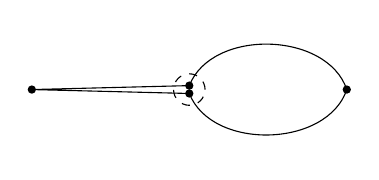
\begin{tikzpicture}
		    \def\r{2}	
		    \def\eps{0.05}
				
		    \coordinate (A) at (-\r,0);
		    \coordinate (B) at (0,\eps);
		    \coordinate (C) at (\r,0);
		    \coordinate (D) at (0,-\eps);
			
		    \draw (D) -- (A) -- (B);
		    \draw (B) to [bend left=70] (C);
		    \draw (D) to [bend right=70] (C);
			
		    \foreach \point in {A,B,C,D}
		        \fill [\vertexColor] (\point) circle (1.5pt);
				
		    \draw [dashed] (0,0) circle (0.2);
                \end{tikzpicture}
            }
        \end{center}
    \end{overlayarea}
\end{frame}


\begin{frame}{How to define abstract folding?}
    \uncover<2->{We need to define two structures:}
    \begin{enumerate}
        \item<3-> A folding state
            \begin{itemize}
                \item<5-> Based on polygonal complexes
                \item<6-> Describe ``is folded together" by an equivalence relation
                \item<7-> Describe order of faces in folding state
            \end{itemize}
        \item<4-> The folding steps
            \begin{itemize}
                \item<8-> Explain ``unordered folding" (e.\,g. covering)
                \item<9-> Modify to include face order relations
            \end{itemize}
    \end{enumerate}
\end{frame}



